\documentclass[output=paper,colorlinks,citecolor=brown,nonflat]{../langscibook}
\author{Laura Sánchez\affiliation{Stockholms universitet}}
\title{Multilingualism from a language acquisition perspective}
\abstract{This chapter conceptualizes and discusses two subtypes of multilingualism, namely, a) third language acquisition in learners who have prior experience in acquiring one or more non-native languages and b) subsequent language acquisition in learners who are bilingual from an early age. The chapter also discusses the roles played by age (both biological age and age of onset) and proficiency in multilingual acquisition. As regards age, the discussion focuses primarily on two aspects, namely, differential effects in instructed and naturalistic contexts, and the apparent superiority of older learners and late starters against younger learners and early starters. It is stressed that further research is necessary in order to identify and single out the particularities of L3 acquisition for learners with prior experience in the concurrent or consecutive learning of one or more non-native languages. Likewise, the chapter highlights the need to obtain a deeper understanding of how age-related differences in the level of linguistic entrenchment in multilinguals constrain L3 learning after exposure to additional languages. With respect to the proficiency factor, it is argued that it is important to consider proficiency thresholds and to tease apart the distinctive effects of proficiency in the target language (the L3) and in the background languages when exploring linguistic development among multilinguals. These distinctive effects are also relevant for understanding crosslinguistic influence in L3 acquisition, above all in determining the potential source languages and the direction of this influence.}
\epigram{The art of language learning may lie not in the acquisition of an individual language but in the mastery of the learning process itself}
\epigramsource{\citep[201]{Tonkin2009}}


\begin{document}
\maketitle



\section{Definitions of multilingualism and third (or additional) language acquisition}\label{sec:sanchez1:1}

In present days, to claim that “multilingualism is no longer the exception but the rule” \citep[113]{Sánchez2019CLIL} may seem uncontroversial. From a terminological point of view, however, defining the term ‘multilingualism’ and distinguishing it from other language contact and learning situations such as bilingualism or second language (L2) acquisition is a different and more complicated matter \citep{Cenoz2013}. A common misconception stems from the lack of clarity when it comes to distinguishing bilingualism and multilingualism and the interchangeable use of the two terms made sometimes in the literature. For example, some authors have defined multilingualism as “the acquisition and use of \textit{two or more} languages” (\citealt[2]{AroninSingleton2008}; emphasis added). By the same token, the term \textit{second language} is sometimes viewed as a “cover term for any language other than the first language learned by a given learner or group of learners irrespective of the type of learning environment and irrespective of the number of other non-native languages possessed by the learner” (\citealt[7]{SharwoodSmith1994}), and the term \textit{bilingual} is used when referring to those “who use two or more languages in their everyday life” (\citealt[xiii]{Grosjean2010}).

Along these lines, \citet[2]{MitchellMyles1998} claim that “it is sensible to include ‘foreign’ languages under our more general term of ‘second’ languages, because we believe that the underlying learning processes are essentially \textit{the same} for more local and more remote target languages, despite differing in learning purposes and circumstances” (emphasis added). Leaving aside other perspectives – such as linguistic, sociolinguistic, or educational–, from an acquisitional perspective, the views and definitions just discussed might be oversimplifications of the situation, failing to acknowledge the distinctive characteristics of multilingualism. Thus, \citet[14]{Cenoz2013} draws attention to the fact that multilingualism is not “a simple addition of languages but a phenomenon with its own characteristics”.

 Inspired by the work of researchers such as \citet{Hufeisen1998, Hufeisen2003} and \citet{DeAngelis2007}, third (or additional) language acquisition (L3) emerged as an independent field of research within multilingualism. As such, L3 acquisition is defined as the learning situation for learners “with prior experience of acquiring one or more non-native languages” (\citealt[128]{Hammarberg2018}). To disseminate research that specifically addresses L3 acquisition, theoretical and empirical papers have started to be regularly presented at seminal conferences and yearly L3 workshops. The dissemination of results from some of these conferences, in the form of (online) publications primarily in English (see \citealt{CenozEtAl2001}) and German\footnote{\url{https://www.daf.tudarmstadt.de/forschungprojekte/laufende_projekte/l3forschung_1/index.en.jsp}{.}} sought to build a case for multilingualism and, especially, for L3 acquisition, by arguing that the underlying learning processes in bi- and tri-and multilingual contexts are not the same. Some of the arguments offered in the literature on multilingualism research are revisited in the following paragraphs.

Problematizing how to define bilingualism and multilingualism seems necessary in order to move forward to a more rigorous and perhaps more accurate view of language acquisition in multilingual learners. At the core of the arguments used to defend the idea that the L2 and L3 learning processes are essentially not “the same” (contrary to \citealt{MitchellMyles1998}) is the belief that there are meaningful differences between the acquisition of an L2 and the acquisition of an L3. Before addressing these differences in more depth, a definition of what is understood as ‘L2’ and ‘L3’ in this chapter is offered. For a start, the working definition of L2 here resonates with \citegen[61]{FalkBardel2010} claim that a true L2 corresponds to “the first encounter with a non-native language” (but see also the definition of ‘L2’ in \sectref{sec:sanchez1:1.2}). In turn, the L3 is defined as any language “beyond the L2 without giving preference to any particular language” (\citealt[11]{DeAngelis2007}), because the critical difference is between the acquisition of an L2 and an L3, but not between an L3 and an L4, L5, L6, etc. (\citealt{Hammarberg2001, Hufeisen2003, DeAngelis2007}). This definition of the L3 is consistent with its status as the \textit{tertiary language} in compliance with proposals in early papers (\citealt{LindemannHufeisen1998, DentlerEtAl2000}) as well as more recent ones \citep{Hammarberg2018}.

\subsection{Prior language learning experiences and strategies in L3 acquisition}\label{sec:sanchez1:1.1}

The belief that there are meaningful differences between the acquisition of an L2 and that of an L3 has its roots in the so-called “difference assumption” position, which is contrary to the “no difference assumption” (\citealt{DeAngelis2007}) represented by the bilingual bias endorsed in the views above (\citealt{SharwoodSmith1994, MitchellMyles1998, Grosjean2010}). Within the difference assumption position, this belief is anchored in the fact that prior knowledge and, above all, prior learning experience have a big impact on the acquisition of an L3. The critical point that differentiates the acquisition of an L2 from that of an L3 is the presence, at the onset of L3 acquisition, of language-specific learning experiences, knowledge and strategies (\citealt{GibsonHufeisen2003}) that beginning learners of a first foreign language do not yet have. As \citet[145]{MarxHufeisen2004} put it, “the addition of further languages changes the language acquisition process not only quantitatively (especially moving from L2 to L3) but – more importantly– qualitatively”.

Similarly, \citet[207]{Jessner1999} points out that “prior language learning experience changes the quality of language learning”, and \citet[14]{Jessner2006} elaborates on this idea by proposing that “the \textit{process of learning} and \textit{the product of having learnt a second language} can potentially exert influence on the acquisition of an L3 and this involves a quality change in language learning and processing” (emphasis added). The qualitative change proposed by Hufeisen in different papers is represented in \figref{fig:sanchez1:1} (\citealt{Hufeisen1998}, also \citealt[145]{MarxHufeisen2004}), adapted from \citet[314]{HufeisenMarx2007}.

% \begin{figure}
%     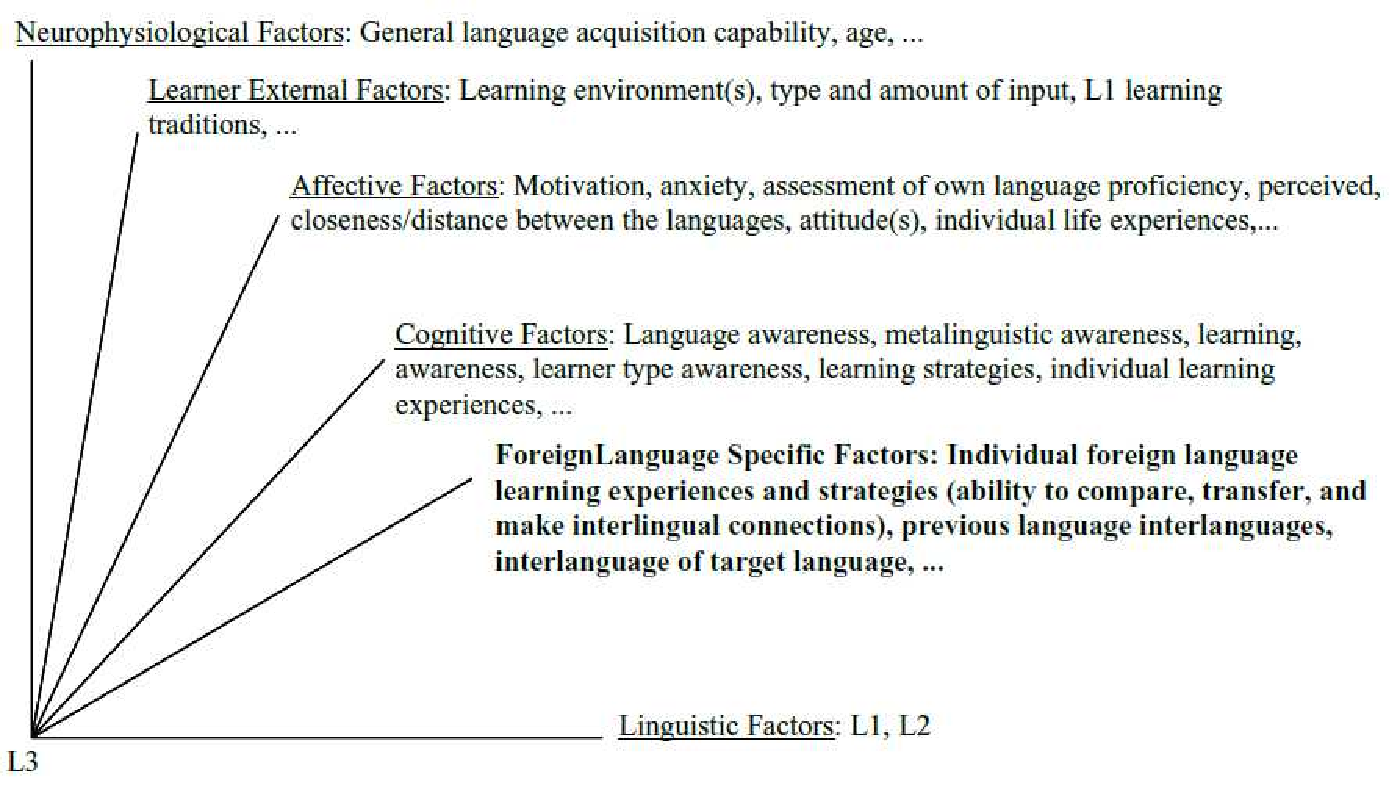
\includegraphics[width=\textwidth]{figures/Sanchez1 Figure 1.pdf}
%     \caption{Third language acquisition (L2 vs. L3)\footnote{Figure reproduced with permission of the author and the publisher.}}
%     \label{fig:sanchez1:1}
% \end{figure}

%Requires some fine tuning!

\begin{figure}
\begin{forest}
  for tree={forked edges, grow'=0, child anchor=west, align=left}
  [ L3, calign=last
    [ {\uline{Neurophysiological factors}: General language acquisition capability, age, ...},tier=x ]
    [ {\uline{Learner external factors}: Learning environment(s), type \\and amount of input, L1 learning traditions, ...},tier=x ]
    [ {\uline{Affective factors}: Motivation, anxiety, \\
    assessment of own language proficiency, \\
    perceived, closeness/distance between the \\
    languages, attitude(s), individual life \\
    experiences, ...},tier=x ]
    [ {\uline{Cognitive factors}: Language awareness, \\
    metalinguistic awareness, learning, \\
    awareness, learner type awareness, \\
    learning strategies, individual \\
    learning experiences, ...},tier=x ]
    [ {Foreign language specific factors: \\
    Individual foreign language learning \\
    experiences and strategies (ability to \\
    compare, transfer, and make interlingual \\
    connections), previous language \\
    interlanguages, interlanguage of \\
    target language, ...},tier=x ]
    [ {\uline{Linguistic factors}: L1, L2}]
  ]
\end{forest}
\caption{Third language acquisition (L2 vs. L3)\label{fig:sanchez1:1}}
\end{figure}

The figure includes factors that are commonly investigated in bilingual and L2 acquisition research, especially from the individual differences framework that underlies much work in the field at present (e.g. \citealt{KiddEtAl2018}). These individual differences (especially neurophysiological and affective ones identified in \figref{fig:sanchez1:1}) embrace, but are not limited to, age, proficiency, aptitude or motivation, which are factors frequently cited in the literature when explaining, for example, linguistic development and ultimate attainment. More importantly, the figure also incorporates foreign language specific factors such as previous interlanguages that configure the acquisition of an L3 in a multilingual learning situation. The extent to which the meaningful and qualitative differences portrayed here might indeed lead to a fundamental distinction between L2 and L3 acquisition, as outlined earlier in this section, might possibly be confirmed in future investigations, and nowadays it constitutes a well-established, thought-provoking, and productive line of investigation.

In research on multilingualism, the prominent role of L2 prior language knowledge, experiences and strategies has also been highlighted in other studies that try to relate language learning experience with a number of benefits in the acquisition process. In discussing experiments conducted with multilingual learners, \citet[35]{Sanz2000} claims that language learning experience “contributes to the automatization of basic subskills involved in input processing and frees up resources that can be devoted to focus on form”. Moreover, prior language learning experience sensitizes multilingual learners to triggering data in the input they receive (\citealt{Zobl1992, Klein1995}).

One reason why language learning experience turns into an asset for multilingual learners is, according to \citet[6]{McLaughlinNayak1989} that the process of language learning “carries over to the learning of a new language”. After all, as the opening quotation suggests, success in language learning very much depends on the mastery of the learning process. Above all, this carrying over takes place by building up certain basic skills that positively transfer to new language learning situations. This process would, in turn, relate to the learning of \textit{routines} (\citealt[360]{Jessner2008Knowledge}; \citealt[804]{RutgersEvans2017}), especially of complex skills. In the process of language learning, routines are important because they are part of the explicit knowledge that is sustained by declarative memory (\citealt{Paradis2009, SharwoodSmith2010, TagarelliEtAl2011}). Learners access this knowledge during sentence construction in non-native languages, and rely on linguistic routines that are stored in memory and that carry out working memory functions (\citealt{BaarsFranklin2003, SharwoodSmith2010}). In the understanding that repeated practice leads to proceduralization, as suggested in skill acquisition theory (\citealt{DeKeyser2007,DeKeyser2010}), what becomes proceduralized or automatized are the implicit computational procedures. Along similar lines, \citet{RutgersEvans2017} claim that what becomes automatized are precisely the linguistic routines that involve controlled processing.

From this viewpoint, once these routines and procedures are consolidated and become automatized, learners are believed to benefit from ‘metaprocedural’ gains from the learning of languages that trigger a more effective restructuring of internal representations (\citealt{McLaughlinNayak1989, NayakEtAl1990}). These metaprocedural gains also help multilingual learners have a greater cognitive flexibility in switching strategies and a greater variety in strategy use (\citealt{Missler2000, Kemp2007}). Such strategy use is assumed to heighten language awareness \citep{Thomas1992}, which serves as a resource to build new knowledge. By so doing, strategy use and language awareness prompt multilinguals to think in a more abstract manner, and enable them to allocate processing resources in a more efficient way under different implicit and explicit learning conditions (\citealt{NationMcLaughlin1986}), especially as far as inductive learning is concerned involving rule discovery \citep{NayakEtAl1990}.

Another way in which prior language knowledge becomes an asset for multilingual learners could be that “experience with a number of languages may make the individual more aware of structural similarities and differences” (\citealt[11]{McLaughlinNayak1989}). Though the facilitative effects of similarities are generally acknowledged (\citealt{Ringbom2007, RutgersEvans2017}; but see \citealt{SwainEtAl1990} and \citealt{GibsonEtAl2001}), especially in the case of cognates \citepv{chapters/munoz}, it might also be the case that multilingual learners may be suspicious of strong (objective or perceived) similarities between two or more languages in their linguistic repertoire (\citealt{Fouser2001, OtwinowskaSzewczyk2017}) or even that certain similarities would have a temporary compromising effect on underdeveloped interlanguage(s) in L3 learners (\citealt{BardelFalk2007, Rast2010, Sánchez2012,chapters/sanchez7} [this volume]).

When discussing the role of prior language experience, \citet{Jessner1999} pinpoints the advantages gained from contact with several languages and argues that such contact has “catalytic effects” (p. 203) on the learning of an L3. It must be noted, however, that it is not entirely clear to what extent the benefits observed in multilinguals are caused by a more effective strategy use, or merely by language learning experience per se, which involves skills that are developed “on account of the demands of processing multiple languages” \citep[243]{Kemp2007}. In relation to L3 writing, for example, it has been found that learners rely on procedural language skills that reflect experience-based monitoring of which they are not necessarily aware (\citealt{RutgersEvans2017}).

\subsection{Multilingual language acquisition in bilingual contexts}\label{sec:sanchez1:1.2}

The role of prior linguistic experience in multilingualism has also been examined in situations where early bilingual learners acquire another language, i.e., a subtype of multilingualism that is different from the type depicted in the preceding section. So far the description of multilingualism has revolved around L3 acquisition by learners with prior experience of acquiring one or more non-native languages. This is the type of multilingualism examined in several of the chapters included in the current edited volume (\citeauthor{chapters/gudmundson, chapters/salaberry, chapters/sanchez7, chapters/sciutti} and \citeauthor{chapters/stadt}).

At this point we shift gears to another multilingual scenario where bilingual children acquire a new language, which would be the language number three (L3) in their linguistic repertoire and their first foreign language. In other words, the criterion according to which this language is an L3 is a chronological one, and as such, it needs to be distinguished and differentiated from the definition above as any language beyond the L2, that is, beyond the first non-native language (see also \citetv{chapters/munoz} and \citetv{chapters/pfenninger}).

Research on this subtype of multilingualism has been conducted with learners from disparate language backgrounds and with disparate linguistic histories. In the case of Europe, two common scenarios emerge. In one of them simultaneous bilinguals are investigated, as in Catalonia with Spanish and Catalan (\citealt{Muñoz2000, Muñoz2000}). This is similar to the case of Spanish-Basque bilinguals in the Basque Country (\citealt{García-MayoGarcía-Lecumberri2003}). In both of these contexts, where bilingualism of two official (majority and minority) languages has additive linguistic consequences (\citealt{CenozValencia1994, Sanz2000}), the next language to be learnt is English, which is the first foreign language, and an obligatory school subject from the age of eight. The other scenario investigates the acquisition of English as a first foreign language on the part of early (from birth) bilinguals and late (newly arrived) bilinguals who speak the community language and a heritage language at home.

Irrespective of the type of bilingualism investigated in these scenarios, the primary aim of these studies has been to demonstrate whether prior linguistic experience enhances subsequent language acquisition. On this subject, it has been suggested that bilinguals have an advantage over monolinguals when it comes to the acquisition of an L3 (\citealt{Sanz2000, Cenoz2003, Cenoz2013, Kopečková2016, HiroshiDegani2018}), though mixed results have been reported. Among others, a possible explanation for mixed results is the large variation in the methodologies employed in these studies, from the participants’ linguistic profile and socioeconomic status to the instruments employed in the data collection. Another plausible explanation is that bilingualism may not have advantages across the board for subsequent language learning, and its benefits may be constrained by the language area (e.g. lexis or syntax) or linguistic skill (e.g. reading or writing).

Counter to what was believed in the 60s and the 70s, where bilingualism was thought to have a detrimental effect on language development, some studies have claimed that both active and passive bilingualism seem to contribute positively to the acquisition of a subsequent language (\citealt{CenozValencia1994, Muñoz2000, Sanz2000, Brohy2001}), but also note studies reporting no effect (\citealt{JaspaertLemmens1990, SandersMeijers1995}). The positive contribution has been found even when the learners are not literate in one of their L1s \citep{WagnerEtAl1989}, in contrast with the small contribution reported in contexts of higher socioeconomic status (\citealt{BenmamounEtAl2013, Polinsky2015}). The main argument put forward in trying to explain the positive contribution of bilingualism to subsequent language acquisition is the transfer of prior knowledge, skills and processing routines. This interpretation is consistent with \citeapo{Cummins1981} linguistic interdependence hypothesis for the transferability of literacy skills from the L1, and it reinforces the role played by prior language experience in multilingualism.

In more or less direct ways, the outcomes of language learning in multilingual settings are always interpreted in the light of two factors, namely age and proficiency. These two factors are reviewed in sections \ref{sec:sanchez1:2} and \ref{sec:sanchez1:3}, respectively. Of course an extensive review of findings related to these factors is beyond the scope of the present chapter. Hence, the following sections try to offer a succinct outline of general findings in relation to age and proficiency, and then move on to discuss some issues more directly related to effects on multilingual language acquisition.

\section{The age factor in multilingual language acquisition}\label{sec:sanchez1:2}

Age is one of the most widely investigated factors in the literature on L2 acquisition (see recent reviews in \citealt{PfenningerSingleton2017, SingletonPfenninger2018, Muñoz2019, MuñozSingleton2019}). While much work has been done to determine the effects of both biological (age-at-time-of-testing) and starting age (age at the onset of target language acquisition) when it comes to the acquisition of an L2, much less work has been carried out to specifically examine the complex ways in which age and additional language acquisition relate to each other. As \citet[433]{Muñoz2019} notices, a very early exposure to an additional language in pre-primary school is “expected to open children’s minds to multilingualism”. Moreover, although the starting ages for a first and a second foreign language are important, above all insofar as they have a bearing on the particular sequence in which they should be taught at school (\citealt[222]{MuñozSingleton2019}), very little evidence is available on how starting and biological age impacts the concurrent acquisition of two foreign languages. Thus, further evidence is needed of the effects of starting age on L3 acquisition in its definition as any language beyond the L2 or first foreign language. Rather, the evidence available in multilingualism research is informed by bilingual learners, often immigrants, learning their first foreign language in a variety of contexts, as indicated in the scenarios described at the beginning of \sectref{sec:sanchez1:1.2}. Consequently, more research is needed in order to identify and single out the particularities of L3 acquisition for learners with prior experience in acquiring one or more non-native languages. Such research may focus on obtaining a deeper understanding of the differences between early and late multilinguals in the level of linguistic entrenchment before they are exposed to subsequent languages, and also the consequences of this entrenchment for multilingualism, especially in cases involving the acquisition of two or more non-native languages at the same time.

One important fact that needs to be considered when discussing age effects on multilingualism is that such effects differ according to the learning environment. A distinction needs to be made between formal or instructed acquisition at school, and acquisition in naturalistic settings \citep{Bardel2019}. While age effects have been investigated in terms of acquisition rate and ultimate attainment (nativelikeness) in both contexts, ultimate attainment could be said to have been more thoroughly investigated in naturalistic settings. The discussion here then is confined to relevant findings in relation to rate and success (efficiency) of foreign language learning.

For the purposes of this chapter, the effects of age on the rate and success of bilingual learners in multilingual language acquisition are largely grounded in the results obtained by the BAF\footnote{ \textrm{‘Barcelona Age Factor’ Project.}} project in Catalonia. The project investigated the instructed acquisition of English as a first foreign language in over 1000 primary and secondary school learners who were bilingual in Spanish and Catalan to different extents (for a detailed description, see \citealt{Muñoz2000}). This large- scale study was longitudinal and relied on a large battery of tests that measured the learners’ general proficiency and their proficiency in specific areas (i.e. dictation, cloze test, listening comprehension, grammar multiple choice test, written composition, oral narrative, oral interview, phonetic imitation, phonetic discrimination, and role-play).

The main goal of the project was to investigate the effects in the short and medium-terms of biological and starting age on the formal acquisition of English as a foreign language at primary and secondary schools. To this aim, data were compared from learners who had begun learning English at different ages (i.e. 8 and 11) but had received the same amount of instruction (200, 416 and 726 hours of instruction). At the time of data collection, the mean ages of the three groups of early starters were 10.9, 12.9 and 16.9, whereas the mean ages of the late starters were 12.9, 14.9 and 17.9, respectively. The main results of the project are gathered in \citegen{Muñoz2006} edited volume, which summarizes the most important findings. The most general conclusion was that late starters (that is, those who started at age 11 instead of at age 8) and older learners (in terms of biological age) had at least an initial advantage over early starters and younger learners. These results were consistent with those obtained in a comparable learning situation, namely, the Basque Country, with bilingual learners (Spanish and Basque) of English as a first foreign language at school (\citealt{García-MayoGarcía-Lecumberri2003}). The data analysed by researchers in the Basque Country came from learners who were roughly the same ages as in Catalonia, but the amount and length of instruction received by those learners were slightly different (e.g. 310, 396, 594, 600, 693, or 792 hours of instruction).

Crucially, the results in Catalonia and the Basque Country have been echoed in different multilingual contexts such as Switzerland. \citet{Pfenninger2014} and \citet{PfenningerSingleton2017, PfenningerSingleton2019}, in another large scale study, investigated bilingual learners in Switzerland who spoke the community language, Swiss German, and another language at home. The starting age for the learners in these studies was similar to those in the studies discussed above (8--9), but the late starters had started at a somewhat later age (i.e. when they were 13-14 years old). Data were collected longitudinally at different points in time. At the first data collection period, early starters had received 440 hours of instruction over 5.5 years and late starters 50 hours of instruction over the course of only six months. The second data collection took place five years later when the learners were 18-19 years old and had received an additional 650 hours of instruction. In this case, the findings also conceded an advantage to older learners, and this was so in spite of the greater length and amount of instruction in the case of early starters.

In none of the multilingual learning contexts discussed here was there clear-cut evidence that early starters would catch up with late starters in the long run. Summing up, the various studies in these different multilingual instructional settings come to the same results. First of all, it seems that older learners, who have undergone greater cognitive development and have higher metalinguistic awareness, outperform their younger peers when learning their first foreign language (L3 English). Moreover, this superiority is manifestly conspicuous in the area of morphosyntax (lending support to the findings reported for bilinguals in \citealt{KrashenEtAl1979}). In contrast, younger learners and early starters, who are at a different stage of maturity, are less efficient learners and their rate of acquisition of the L3 is slower.

Another important conclusion reached in these studies is that age alone cannot tell the whole story. More precisely, these studies have found that input is as important as, or even more so, than age (\citealt{Muñoz2006, Muñoz2014, Muñoz2019, PfenningerSingleton2017}) not only in terms of amount but also of type. Interestingly, input through exposure at school is neither the only nor the most important source of input for these learners. Instead, it seems that they engage in many extramural English activities, which corroborates the idea of such activities benefitting foreign language learning advanced in other studies (\citealt{SundqvistSylvén2014}). These activities range from simply surfing on the internet and watching TV (with or without subtitles), to reading and engaging in digital gameplay, and they seem to make a significant contribution to the acquisition of English as a foreign language, especially to the growth of vocabulary and the development of oral abilities. Besides amount and type of input, it is apparent that age is interrelated with other factors as well \citep{Muñoz2014}, and a few studies have revealed the robust effects of parental education and literacy skills (\citealt{PfenningerSingleton2017, Muñoz2019, MuñozSingleton2019}). Similar results on parental education and literacy skills were obtained in a study with 14-year-old learners of L3 English with L1 Italian and L2 German (\citealt{DeAngelis2015}).

Another relevant interrelation is that between age and L3 proficiency. Hence, due to the interrelation of these two factors, age-related variation in learning rate allows older and younger learners to benefit from instruction to different extents \citep{Muñoz2006}, because proficiency does not necessarily reflect amount of instruction. In a study on the acquisition of L3 German by Swedish learners with prior knowledge of L2 English, \citet{Sayehli2001} found that some of her 12--13 year-olds were of overall higher proficiency than 13-14 year-olds. The fact that the proficiency level of some of the less instructed learners was higher than that of their more instructed peers was explained as a result of this lack of correspondence between proficiency and amount of instruction. An important implication of this mismatch, as argued by \citet[214]{MuñozSingleton2019}, is that “the degrees of proficiency attained by multilingual school learners are influenced by the age at which they begin to learn the additional language”.

\section{The proficiency factor in multilingual language acquisition}\label{sec:sanchez1:3}

The preceding section has addressed the role of proficiency as regards its interaction with age in explaining success in foreign language acquisition. In turn, this section addresses the role of the proficiency factor in multilingual language acquisition. Another important yet difficult question to ask then is at what stage of development in the target language, the L3, learners benefit the most from their prior linguistic knowledge. Indeed, the question is essential if one considers that language learning beyond the L2 brings about the activation of the entire array of competences of multilingual speakers \citep{Coste1997}, thereby enhancing their degree of metalinguistic awareness \citep{Jessner2008Knowledge}. In the case of bilingual learners acquiring a subsequent language, \citet{Cenoz2013} discusses evidence suggesting that at intermediate proficiency levels in the L3, prior language knowledge is facilitative.

In the case of L3 language acquisition, \citet[34]{DeAngelis2007} has stressed the need to “address the question of threshold levels, in other words how proficient learners need to be before their prior knowledge begins to affect the production and development of a target language to a significant extent”. The need to investigate proficiency in all the languages of a multilingual learner is central to a prolific research branch within multilingualism, namely, crosslinguistic influence (see \sectref{sec:sanchez1:4}). Thus, research on crosslinguistic influence in multilingual language acquisition points out the importance of teasing apart the differential effects of proficiency in the target language (the L3) and proficiency in background languages that can become potential source languages of influence (e.g. \citealt{BardelLindqvist2007, DeAngelis2007, FalkBardel2010, Jaensch2011, LindqvistBardel2013, SánchezBardel2016}). For recent overviews of the role of proficiency in the target language (L3) and source language of influence (L2) on the occurrence of crosslinguistic influence in multilingual learners see \citet{Sánchez2014} and \citet{SánchezBardel2017}, respectively.

A distinguishing feature of proficiency in L3 acquisition is that “from a methodological perspective, information on proficiency level in previously acquired non-native languages is central to be able to establish a distinction between the L2 and the multilingual learner, and consequently between second language acquisition and third language acquisition” (\citealt[34]{DeAngelis2007}). Hence, it seems wise to define what proficiency in the L2 and the L3 refers to in each case and how the construct is operationalized. To be able to have an adequate understanding of the dynamics of proficiency in multilingualism, the definition must embrace the unique characteristics of multilingual language acquisition and capture the essence of its distinctiveness. In this endeavor, two terms that have been proposed are ‘multicompetence’ \citep{Cook1995} and ‘multilingual proficiency’.

Within the multicompetence framework, proficiency is seen as a whole and reflects the interaction between proficiencies (L1, L2, L3) in the mind of the learner, highlighting that the competence of multilinguals is different from that of monolinguals in the same way as the competence of bilinguals is different from that of monolinguals \citep{Grosjean2001}. In turn, multilingual proficiency views proficiency as a “cumulative measure” of the various subcomponents (lexical, syntactic and phonetic) of each “language system” (i.e. background language) of the multilingual (\citealt[109]{HerdinaJessner2002}), with some deviations from the expected language norm to be attributed to the “interaction” between the different language systems (p. 127). More importantly, within the dynamic model of multilingualism (\citealt{HerdinaJessner2002, Jessner2008Knowledge}), proficiency is presumed to operate under the auspices of the so-called “M-factor” (multilingualism factor), an emergent property that “can be specified as a function of the interaction between more than one language system” (\citealt[130]{HerdinaJessner2002}). Moreover, the authors claim, “[i]t is not necessarily relevant how these language systems develop, but may be dependent upon the number of language systems involved”. Because of this interaction of proficiencies, multilinguals are expected to perform differently from bilinguals and L2 learners \citep{Stratilaki2006}. In this respect, both multicompetence and multilingual proficiency are consistent with the idea of plurilingual competence and encompass a “composite competence” (\citealt[260]{CE2001}), while highlighting the varying and uneven degrees of proficiency in each language of the multilingual \citep{Coste1997}.

The interaction of proficiencies in multilinguals is not a new idea. In fact, it has been proposed that proficiency thresholds between non-native languages (L2 and L3) affect linguistic development in all the languages of a multilingual (\citealt{DeAngelisSelinker2001}). \citet{Cenoz2000} warns that different areas of proficiency in the L1 and the L2 may have a specific effect on different areas of proficiency in the L3. In addition to this, she poses the question whether proficiency in other languages may be influential at all stages of the acquisition of a given L3. An important contribution to research on proficiency thresholds in L3 acquisition are the studies by \citeauthor{Jaensch2011} (e.g. \citeyear{Jaensch2011}), who found a correlation between L2 morphological proficiency (measured in terms of inflection suppliance on adjectives) and the use of inflected adjectives in the L3. Along similar lines, \citet{Trévisiol2006} found a differential effect for proficiency in the L1 and the L2 and their effect on L3 development. Whereas both the L1 (English, typologically closer to the L3s French and Italian) and the L2 (German) were equally likely to affect the L3 at low levels in this language, a proficiency-related developmental shift happened with increasing proficiency in the L3. In particular, the L1 but not the L2 had an effect on the acquisition of the L3 at higher levels of proficiency in the L3.

Another insight into the role of proficiency in multilingualism has to do with how proficiency level may affect lexico-semantic organization in L3 learners. Extending research on bilinguals to research on multilinguals, it has been suggested that proficiency mediates how lexical structure is connected between the mother tongue and non-native languages. In particular, a hypothesis that has received substantial empirical support is that lexical structure between the L1 and a weak foreign language (often the L3) is one of word association, whereas the lexical structure between the L1 and a strong foreign language (often the L2) is one of concept mediation (\citealt{Abunuwara1992, Schönpflug2000, Herwig2001, CenozEtAl2003}). Based on evidence coming from various language combinations and analyzed using different instruments (e.g. Stroop interference test, story-telling task, translation, think-aloud protocol), the tentative conclusions drawn in these studies is that multilinguals’ lexical organization shows a proficiency-related effect, that this organization changes over time as a function of adjustments in L2 and L3 proficiency, and that access in multilinguals is non-selective (\citealt{DijkstraVanHell2003}).

\section{Crosslinguistic influence in L3 acquisition}\label{sec:sanchez1:4}

One area of investigation within multilingualism research that has attracted much attention is crosslinguistic influence. From an L3 acquisition perspective, transfer or crosslinguistic influence is defined as a “largely unconscious interaction phenomenon between evolving sets of imperfectly acquired structures” \citep[143]{Bouvy2000}. The term ‘crosslinguistic interaction’ (\citealt{HerdinaJessner2002, Jessner2003}) subsumes crosslinguistic influence together with other, more conscious phenomena that take place in multilingual environments such as codeswitching and borrowing.

  In addition to the body of articles and book chapters devoted to the investigation of crosslinguistic influence in multilingual language acquisition, several compilations on the topic have been published in recent years, often with a focus on L3 acquisition. Some of them address psycholinguistic and processing issues with a focus on transfer at the level of lexis, phonology and morphology (\citealt{DeAngelisEtAl2015, Peukert2015}). Equally, several studies focus on crosslinguistic influence in the area of syntax (\citealt{Leung2009, CabrelliEtAl2012, AngelovskaHahn2017}), mainly from a generative research perspective.

In the field of L3 acquisition, the investigation of crosslinguistic influence is more complex than in L2 acquisition because this influence involves necessarily more than two languages, often non-native. Empirical studies on crosslinguistic influence involving more than two languages were already conducted in the sixties and the seventies. Despite this early interest in crosslinguistic influence, it was not until the turn of the century (e.g. \citealt{WilliamsHammarberg1998, CenozEtAl2001}) that crosslinguistic influence in such contexts was studied in a more systematic way, meaning that all languages in the learners’ linguistic backgrounds were identified and mentioned and prior non-native languages were given their appropriate status.

A major concern in research on crosslinguistic influence in L3 acquisition has been to try and determine whether it is the L1 or the L2 that acts as the main source language of influence, or whether other characteristics of the background languages (such as close typological relatedness, for instance), determine the degree to which one language will influence another. Another concern is the distinction between different kinds of crosslinguistic influence in L3 acquisition depending on the direction of the influence. The most widely investigated kind is the one that occurs between two non-native languages, usually referred to as ‘interlanguage transfer’ (\citealt{DeAngelisSelinker2001}). Another kind of crosslinguistic influence is the one that takes place from the L2 or the L3 back onto the L1 (\citealt{KecskesPapp2000}), also referred to as “reverse” or “backward” transfer.

Different hypotheses have been put forward about which background language of the multilingual learner is more likely than another to act as the source for crosslinguistic influence. The status of the background language (L1 or L2) has been emphasized in two models that hypothesize the primacy of either a prior non-native language or the mother tongue. The former model is referred to as the L2 status factor hypothesis (\citealt{BardelFalk2007, BardelFalk2012, FalkBardel2010, BardelSánchez2017}). Furthermore, following the premise that a prior L2 is a more likely candidate as a source language of influence, \citet{BardelSánchez2017} discuss empirical evidence suggesting that L3 learners with lower cognitive abilities are less efficient in inhibiting non-intended activation and transfer from the L2 (\citealt{SánchezBardel2016, Sánchez2019Complexity}). They use this evidence to suggest that cognitive factors play a role in the occurrence of crosslinguistic influence in L3 acquisition. Therefore, the authors argue, it is necessary to take into consideration to what extent the amount (but not the quality) of this influence might be explained by differences in cognitive abilities such as working memory capacity and attention control. All in all, the L2 status hypothesis has received much more empirical support than the second hypothesis, the L1 transfer hypothesis (\citealt{NaRanongLeung2009, Hermas2010}), and it has been tested with a wider variety of language combinations. According to the L1 hypothesis, the L1 has a “privileged” role in, at least, the acquisition of L3 subtle syntactic properties, as for example in argument selection (as in these two studies). Hence, when coping with such structures, L3 learners would resort to their L1 underlying grammatical knowledge, rather than to their L2 explicit conscious knowledge (\citealt[185]{NaRanongLeung2009}; \citealt[358]{Hermas2010}).

Rather than status, other proposals consider structural similarity and accumulated language experience to be more important factors. In the typological primacy model \citep{Rothman2015} and the linguistic proximity model \citep{WestergaardEtAl2017}, it is claimed that the most likely source language of influence will be the background language that more closely resembles the L3. The cumulative enhancement model for language acquisition, in turn, claims that “experience in any prior language can be drawn upon in subsequent acquisition” (\citealt[13]{FlynnEtAl2004}) and that crosslinguistic influence has a facilitative effect. Less whole-sale predictions can be made based on the scalpel model \citep{Slabakova2017}, because it envisions crosslinguistic influence to work property by property. As such, crosslinguistic influence would be language-dependent, and it would be shaped by factors “such as construction frequency, availability of clear unambiguous input, prevalent use and structural linguistic complexity, among others” \citep[653]{Slabakova2017}. Due to limitations of space, a more comprehensive reexamination of these and other studies is not possible in the concise set up of the scene here. Hopefully, however, these lines will serve a useful point of departure for the interested reader. For recent overviews of findings in research on crosslinguistic influence in L3 acquisition, the reader is directed to the reviews in \citet{Bardel2019, DeAngelis2019} and \citet{Puig-MayencoEtAl2018}.

\section{Conclusions}\label{sec:sanchez1:5}

The present theoretical chapter has attempted to offer an overall picture of multilingual acquisition, while emphasizing the need to distinguish it from other language learning situations where only two languages are in contact. With this as the starting point, the discussion has proposed a fine-grained distinction between the two most common types of multilingual acquisition described in the literature, especially with regard to third language acquisition. Firstly, the case of third language acquisition in learners who have prior experience in acquiring one or more non-native languages. Secondly, the case of subsequent acquisition in learners who are bilingual from an early age. In order to have a better understanding of the dynamics of language acquisition in such multilingual contexts, it is necessary to take into account the effects that an earlier or later onset in the L1 and the L2 may have on development and learning in the L3. At the same time, it is also necessary to consider the asymmetries in the proficiency level of all the languages of the multilingual learner, and how they constrain and shape subsequent language acquisition. Finally, this chapter has given a grasp of current research on crosslinguistic influence in third language acquisition, with a focus on how native and non-native languages interact in the mind of the multilingual learner, and what the consequences of this interaction are for interlanguage development in the acquisition of a third or additional language.

\sloppy\printbibliography[heading=subbibliography,notkeyword=this]
\end{document}
